\hypertarget{a00340}{}\section{Direct Memory Access}
\label{a00340}\index{Direct Memory Access@{Direct Memory Access}}
D\+M\+A support for A\+A\+X D\+S\+P plug-\/ins, with emulation for A\+A\+X Native. 

\hypertarget{a00340_algdmapagecontents}{}\subsection{On this page}\label{a00340_algdmapagecontents}
\begin{DoxyItemize}
\item \hyperlink{a00340_alg_dma_overview}{D\+M\+A facility overview} \item \hyperlink{a00340_alg_dma_modes}{D\+M\+A transfer modes} \item \hyperlink{a00340_alg_dma_registration}{Registering for D\+M\+A transfers} \item \hyperlink{a00340_alg_dma_restrictions}{D\+M\+A restrictions} \item \hyperlink{a00340_alg_dma_additionalinformation}{Additional information}\end{DoxyItemize}
\hypertarget{a00340_alg_dma_overview}{}\subsection{D\+M\+A facility overview}\label{a00340_alg_dma_overview}
A\+A\+X provides an \hyperlink{a00095}{abstract interface} for accessing the host environment\textquotesingle{}s D\+M\+A or other memory-\/transfer facilities. All platform-\/specific details are handled by the A\+A\+X host environment, allowing plug-\/ins that use this interface to be re-\/targeted to to Native or D\+S\+P environments without changing their memory transfer implementation.\hypertarget{a00340_alg_dma_modes}{}\subsection{D\+M\+A transfer modes}\label{a00340_alg_dma_modes}
A\+A\+X hosts may support the following D\+M\+A modes, as listed in \hyperlink{a00095_af8d0f19f2896dd6dbd126b919b24e39b}{A\+A\+X\+\_\+\+I\+Dma\+::\+E\+Mode} \+:

\begin{DoxyItemize}
\item In \hyperlink{a00095_af8d0f19f2896dd6dbd126b919b24e39bac8f3cbed92bc7d135e306cc154ac2ae6}{Scatter} mode, data is transferred from a linear buffer to a series of offset segments in a circular buffer. This mode is most often used to transfer data from linear internal memory to a large external memory buffer.\end{DoxyItemize}
\begin{DoxyItemize}
\item In \hyperlink{a00095_af8d0f19f2896dd6dbd126b919b24e39badec2b76540ba9a168b7a049acb50654d}{Gather} mode, data is collected from a series of offset segments in a circular buffer and concatenated in a linear buffer. This mode is most often used to transfer data from an external memory buffer to an internal memory buffer.\end{DoxyItemize}
\begin{DoxyItemize}
\item In \hyperlink{a00095_af8d0f19f2896dd6dbd126b919b24e39ba253c129077dc004dd83cca8931e69eb9}{Burst} mode, data is written linearly from one location to another. Burst mode transfers may be used for linear transfers of data to or from external memory. During the transfer, the source data is broken into a series of individual bursts. This mode is included for completeness, though the Scatter/\+Gather modes are expected to be more appropriate for the vast majority of real-\/world D\+M\+A use cases.\end{DoxyItemize}
\hypertarget{a00340_alg_dma_registration}{}\subsection{Registering for D\+M\+A transfers}\label{a00340_alg_dma_registration}
Algorithm Components register for D\+M\+A transfers by adding one or more D\+M\+A fields to their context via \hyperlink{a00088_aff9e1c726bbdf500f2d61b164589744e}{A\+A\+X\+\_\+\+I\+Component\+Descriptor\+::\+Add\+Dma\+Instance()}. At runtime, each field will be populated with a valid \hyperlink{a00095}{D\+M\+A interface} for the specified D\+M\+A mode.\hypertarget{a00340_alg_dma_restrictions}{}\subsection{D\+M\+A restrictions}\label{a00340_alg_dma_restrictions}
The following restrictions apply to D\+M\+A transfers on all A\+A\+X platforms\+:

\begin{DoxyItemize}
\item The maximum burst size for any D\+M\+A transfer is 64\+B. The minimum burst size is 1\+B. \item Only one D\+M\+A transfer request may be posted per \hyperlink{a00095}{A\+A\+X\+\_\+\+I\+Dma} object per processing callback. \item Scatter and Gather requests each require that the circular memory buffer be padded by at least the size of one burst\end{DoxyItemize}
\hypertarget{a00340_alg_dma_additionalinformation}{}\subsection{Additional information}\label{a00340_alg_dma_additionalinformation}
{\bfseries T\+I Guide} \begin{DoxyItemize}
\item \hyperlink{a00362_subsubsection__dma_support_}{D\+M\+A support} \item \hyperlink{a00362_subsubsection__dma_and_background_thread_performance_reporting_}{D\+M\+A and background thread performance reporting} \end{DoxyItemize}
Collaboration diagram for Direct Memory Access\+:
\nopagebreak
\begin{figure}[H]
\begin{center}
\leavevmode
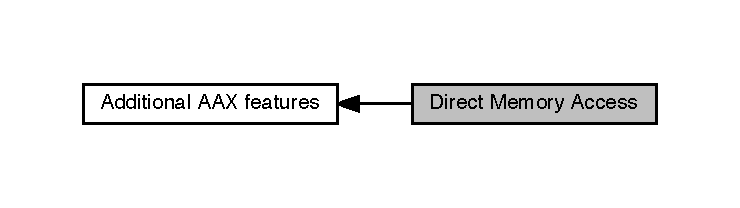
\includegraphics[width=350pt]{a00340}
\end{center}
\end{figure}
